\chapter{Applying Benchmark Reviews to Requirement Decisions}
\label{ch:decisions}

\todo[inline]{Integrate the full content, tables, and verified statistics from \texttt{benchmark-evidence-requirement-decisions/decisions\_paper.tex} (\texttt{main} branch). Cross-reference Appendix~\ref{app:decisions_artifacts} for policy definitions and binomial cut points.}

\section{The Fail-Closed Three-Step Decision Method}
\label{sec:dec_method}

\todo[inline]{Formalize the three-step decision engine: Step~1 (record integrity and SHA-256 provenance of patches and logs), Step~2 (admissibility evaluation of \mesa{} ratings under \texttt{strict}, \texttt{lenient}, and \texttt{controlled} policies plus confirmed defective task filtering), and Step~3 (exact one-sided 95\% binomial bounds yielding Accept, Reject, Inconclusive, or no decision when Step~2 fails).}

\section{Empirical Study Design on SymPy}
\label{sec:dec_design}

Figure~\ref{fig:decisions_overview} outlines the empirical study evaluating one coding agent across 88 SymPy sessions: 44 tasks from \swebench{}~\cite{jimenez_swebench_2024,openai_swebench_verified_2024} and 44 SymPy issues reported and fixed after the agent's reported training cutoff, tested against a 0.70 resolve-rate requirement.

\begin{figure}[htbp]
    \centering
    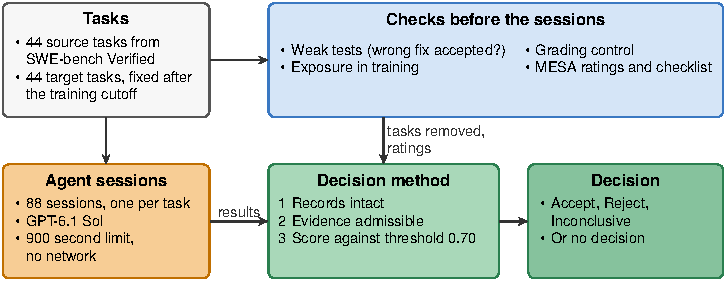
\includegraphics[width=\textwidth]{Figures/decisions_study_overview.pdf}
    \caption{Overview of the Requirement Decisions empirical study: 88 frozen SymPy coding-agent sessions (44 \swebench{} source tasks and 44 post-cutoff target tasks), benchmark and patch validity checks, MESA/ABC ratings, and comparison of seven decision methods.}
    \label{fig:decisions_overview}
\end{figure}

\subsection{Agent Configuration, Task Sets, and Study Freeze}
\label{sec:dec_agent_tasks}

\todo[inline]{Describe the coding agent setup, one attempt and 15-minute limit per issue, offline local repository execution, and frozen study manifests.}

\subsection{Benchmark Checks, Patch Checks, and Review Ratings}
\label{sec:dec_checks_ratings}

\todo[inline]{Describe weak-test counterexample checks, test-runner tampering checks, independent agent patch checks, exposure probes, and completed \mesa{} and Agentic Benchmark Checklist~\cite{zhu_agentic_benchmark_checklist_2025} ratings.}

\subsection{Decision Methods Compared}
\label{sec:dec_methods_compared}

\todo[inline]{Define the seven source decision methods compared on the 44 \swebench{} tasks alongside the direct-test evaluation on the 44 post-cutoff SymPy issues.}

\section{Results}
\label{sec:dec_results}

\subsection{What Each Decision Method Concludes (RQ1)}
\label{sec:dec_rq1}

\todo[inline]{Import verified Table~3 results: 35 of 44 resolved on \swebench{} (79.5\%, Inconclusive under the 0.70 requirement where Accept requires $\ge 37$); test-runner edits passed grading so three methods stopping on failed review items gave no decision; deliberately incomplete patches passed on 32 of 44 tasks; independent patch checks retained 38 tasks (31 resolved, Inconclusive, where Accept requires $\ge 32$), whereas dropping all 32 flagged tasks left only 12 tasks (10 resolved).}

\subsection{Benchmark Tasks Compared with the Post-Cutoff Direct Test (RQ2)}
\label{sec:dec_rq2}

\todo[inline]{Import verified Table~4 results and covariate analysis: 21 of 44 resolved on post-cutoff SymPy issues (47.7\%, Reject under the exact one-sided 95\% upper bound below 0.70); logistic regression covariate analysis of patch size, files touched, issue length, and tests accounting for 15.6 percentage points of the 31.8 percentage-point gap (49\%).}

\subsection{Rule Violations and Session Controls (RQ3)}
\label{sec:dec_rq3}

\todo[inline]{Report observed rule violations, patch-check rejections (0 of 31 source patches vs.\ 3 of 22 target patches), and session integrity checks.}
